%% Copernicus Publications Manuscript Preparation Template for LaTeX Submissions
%% ---------------------------------
%% This template should be used for copernicus.cls
%% The class file and some style files are bundled in the Copernicus Latex Package, which can be downloaded from the different journal webpages.
%% For further assistance please contact Copernicus Publications at: production@copernicus.org
%% https://publications.copernicus.org/for_authors/manuscript_preparation.html

%% copernicus_rticles_template (flag for rticles template detection - do not remove!)

%% Please use the following documentclass and journal abbreviations for discussion papers and final revised papers.

%% 2-column papers and discussion papers
\documentclass[gc, manuscript]{copernicus}



%% Journal abbreviations (please use the same for preprints and final revised papers)

% Advances in Geosciences (adgeo)
% Advances in Radio Science (ars)
% Advances in Science and Research (asr)
% Advances in Statistical Climatology, Meteorology and Oceanography (ascmo)
% Aerosol Research (ar)
% Annales Geophysicae (angeo)
% Archives Animal Breeding (aab)
% Atmospheric Chemistry and Physics (acp)
% Atmospheric Measurement Techniques (amt)
% Biogeosciences (bg)
% Climate of the Past (cp)
% DEUQUA Special Publications (deuquasp)
% Earth Surface Dynamics (esurf)
% Earth System Dynamics (esd)
% Earth System Science Data (essd)
% E&G Quaternary Science Journal (egqsj)
% EGUsphere (egusphere) | This is only for EGUsphere preprints submitted without relation to an EGU journal.
% European Journal of Mineralogy (ejm)
% Fossil Record (fr)
% Geochronology (gchron)
% Geographica Helvetica (gh)
% Geoscience Communication (gc)
% Geoscientific Instrumentation, Methods and Data Systems (gi)
% Geoscientific Model Development (gmd)
% History of Geo- and Space Sciences (hgss)
% Hydrology and Earth System Sciences (hess)
% Journal of Bone and Joint Infection (jbji)
% Journal of Micropalaeontology (jm)
% Journal of Sensors and Sensor Systems (jsss)
% Magnetic Resonance (mr)
% Mechanical Sciences (ms)
% Natural Hazards and Earth System Sciences (nhess)
% Nonlinear Processes in Geophysics (npg)
% Ocean Science (os)
% Polarforschung - Journal of the German Society for Polar Research (polf)
% Primate Biology (pb)
% Proceedings of the International Association of Hydrological Sciences (piahs)
% Safety of Nuclear Waste Disposal (sand)
% Scientific Drilling (sd)
% SOIL (soil)
% Solid Earth (se)
% State of the Planet (sp)
% The Cryosphere (tc)
% Weather and Climate Dynamics (wcd)
% Web Ecology (we)
% Wind Energy Science (wes)

% Pandoc citation processing

% The "Technical instructions for LaTex" by Copernicus require _not_ to insert any additional packages.
% 
% tightlist command for lists without linebreak
\providecommand{\tightlist}{%
  \setlength{\itemsep}{0pt}\setlength{\parskip}{0pt}}


%
\begin{document}


\title{New insights into the Weddell Sea ecosystem applying a
quantitative network approach}


\Author[1, *]{Tomás I.}{Marina}
\Author[1, *]{Leonardo A.}{Saravia}
\Author[2]{Susanne}{Kortsch}


\affil[1]{Centro Austral de Investigaciones Científicas (CADIC-CONICET),
Ushuaia, Argentina}
\affil[2]{Spatial Foodweb Ecology Group, Department of Agricultural
Sciences, University of Helsinki, Finland}
\affil[*]{These authors contributed equally to this work.}

\runningtitle{New insights into the Weddell Sea food web}

\runningauthor{Marina et al.}

\correspondence{Tomás I. Marina (tomasimarina@gmail.com) and Leonardo A.
Saravia (arysar@gmail.com)}


\received{}
\pubdiscuss{} %% only important for two-stage journals
\revised{}
\accepted{}
\published{}

%% These dates will be inserted by Copernicus Publications during the typesetting process.


\firstpage{1}

\maketitle


\begin{abstract}
Network approaches can shed light on the structure and stability of
complex marine communities. In recent years, such approaches have been
successfully applied to study polar ecosystems, improving our knowledge
on how they might respond to ongoing environmental changes. The Weddell
Sea is one of the most studied marine ecosystems outside the Antarctic
Peninsula in the Southern Ocean. Yet, few studies consider the known
complexity of the Weddell Sea food web, which in its current form
comprises 490 species and 16041 predator-prey interactions. Here we
analysed the Weddell Sea food web, focusing on the species and trophic
interactions that underpin ecosystem structure and stability. We
estimated the strength for each interaction in the food web,
characterised species position in the food web using unweighted and
weighted food web properties, and analysed species' roles with respect
to the stability of the food web. We found that the distribution of the
interaction strength (IS) at the food web level is asymmetric, with many
weak interactions and few strong ones. We detected a positive
relationship between species median IS and two unweighted properties
(i.e., trophic level and the total number of interactions). We also
found that only a few species possess key positions in terms of food web
stability. These species are characterised by high median IS, mid to
high trophic level, relatively high number of interactions, and mid to
low trophic similarity. In this study, we integrated unweighted and
weighted food web information, enabling a more complete assessment of
the ecosystem structure and function of the Weddell Sea food web. Our
results provide new insights, which are important for the development of
effective policies and management strategies, particularly given the
ongoing initiative to implement a Marine Protected Area (MPA) in the
Weddell Sea.
\end{abstract}




\introduction[Introduction]

Food web analysis constitutes an important framework for understanding
ecological community structure and for conserving biodiversity through
ecosystem management \citep{Thompson2012}. Although topological food web
analysis, which considers only the presence and absence of predator-prey
interactions, provides important insights into the structure and
functioning of ecological communities
\citep[e.g.][]{Pascual2006, Kortsch2015, Marina2018, Cordone2020, Rodriguez2022},
more information on the nature of the trophic interactions is needed to
effectively characterise ecosystem dynamics and stability
\citep[e.g.][]{Kortsch2021, Pecuchet2022}. This is a fundamental step
for providing assessments on ecosystem vulnerability to environmental
pressures and for prioritising management actions. In this regard,
quantifying the strength of trophic interactions and species' roles
within the network are of paramount importance
\citep{Carrara2015, Allesina2015, Nilsson2016, Cirtwill2018a}.

Estimating interaction strength (IS) in food webs allows differentiating
the importance of species interactions. On the contrary, unweighted food
web representations give equal importance to all interactions
well-knowing that some species interactions are stronger than others and
hence play a different role for ecosystem functioning and stability.
Both empirical and theoretical studies show that interactions strength
distributions in food webs are asymmetric
\citep{Paine1992, McCann1998, Emmerson2004, Wootton2005, Kortsch2021},
containing a few strong and many weak interactions. This asymmetric
patterning of weak and strong links is crucial to food web stability
\citep{Paine1992, McCann1998, Neutel2002}. In a recent paper on an
aquatic food web it was further highlighted that temporal changes in
ecosystem functioning could only be predicted using a weighted food web
structure \citep{Kortsch2021}. Hence, in order to assess the stability
and functioning of a food web, it is important to first determine link
weights.

Several methodologies have been applied to estimate IS in food webs,
where the quantity and quality of the data mostly determine which
approach is the most convenient \citep{Berlow2004}. Approaches include
experimental methods combined with dynamic modelling
\citep{Emmerson2004, Carrara2015}, measurements of species abundances
through time \citep{Fahimipour2014, Chang2021}, and estimation of
metabolic rates and biomass of all species in the community
\citep{Neutel2014}. However, these types of methods require large
experimental set-ups and parameterisations restricting the analyses to
smaller networks (e.g., approximately 10 species or less). Other methods
based on allometric scaling relationships and biomass information
\citep{Kortsch2021, Gauzens2019} can be applied to larger networks with
less data requirements, but this comes at the expense of precision in
the predictions. For even larger food webs composed of nearly 1000
species and more than 10000 interactions, only methods with even less
data requirements are feasible. One of these methods, proposed by
\citet{Pawar2012}, combines data on consumer and resource body masses
and consumer search space (interaction dimensionality) to obtain IS
estimates for each pairwise predator-prey interaction. An advantage of
this method is that it can be applied without information on species
biomass.

Diverse food webs (e.g., terrestrial, lake, marine) from various
geographic locations have been studied worldwide, including marine food
webs in polar regions
\citep{Carscallen2012, Santana2013, Kortsch2019, Pecuchet2022}. Studies
from the Arctic show that marine food web properties (e.g., connectance
and modularity) are constrained by sea ice and seawater temperature
\citep{Kortsch2019, Pecuchet2022}. Likewise for the Southern Ocean it
was shown that sea ice has impacts on local (Ross Sea) food web
structure \citep{Rossi2019}. For example, in the Ross Sea, sea-ice break
up introduced a surge of sympagic food, which led to simpler food webs
with reduced intraguild predation, potential disturbance propagation and
increased vulnerability to biodiversity loss \citep{Rossi2019}.

The Weddell Sea is expected to be one of the last regions of the
Southern Ocean to experience the consequences of climate change due to
its extensive sea ice cover and ocean currents \citep{Teschke2021}
resulting in less sea surface warming compared to other areas of the
Southern Ocean. Generaly, the Southern Ocean plays an important role in
driving global thermohaline circulation and ventilating the global
abyssal ocean because it generates a considerable part of the Antarctic
Bottom Water \citep{Fahrbach2009}. Because of these environmental
characteristics, the Weddell Sea may serve as a refuge for Antarctic
species which depend on sea ice (e.g.~krill, emperor penguin, Weddell
seal) or have low heat tolerance (e.g., most notothenoid fishes) due to
their adaptations to freezing temperatures \citep{Griffiths2017}. While
essential large-scale hydrodynamic relationships are relatively
well-known for this region \citep{deSteur2019}, information on the
current distribution, abundance and sensitivity to climate change is
only partially known for a few species (e.g., emperor penguin)
\citep{Houstin2022}.

The Weddell Sea food web is highly complex, comprising 488 species and
16200 predator-prey interactions \citep{Jacob2011}. To better understand
species roles related to food web stability, Jacob et al.~(2011)
performed secondary extinctions and found that the removal of small to
medium-sized, and not large, organisms caused a cascade of secondary
extinctions. These findings highlighted the relative importance of
predators, rather than prey, for the architecture, functioning and
stability of the Weddell Sea food web, which coincides with findings
from recent meta-analyses in empirical complex food webs
\citep{Brose2019, Perkins2022}. \citet{Brose2019} considered this food
web in a meta-analysis context showing that high predator-prey body-mass
ratios are found for predator groups with specific trait combinations,
including small vertebrates and large swimming or flying predators.
These trait combinations generate weak interactions that stabilize
communities against perturbations maintaining ecosystem functioning.

In this study, we aim to go beyond a purely topological
(presence/absence) assessment of who eats whom in the Weddell Sea
ecosystem by providing a quantitative analysis of the trophic network
structure. We aim to analyse the species' role for the structure and
stability of the food web. To achieve this, we: 1) estimated the
strength for each interaction, 2) characterised species' role
considering both weighted and unweighted properties, and 3) analysed
species' roles related to the stability of the food web.

\section{Methodology}

\subsection{Study area}

The high Antarctic Weddell Sea shelf is situated between 74 and 78ºS,
stretching approximately 450 km from East to West (Figure 1). Water
depth varies between 200 and 500 meters, and shallower areas are covered
by continental ice, which forms the coastline along the eastern and
southern parts of the Weddell Sea. The shelf area contains a complex
three-dimensional benthic habitat with large benthic biomasses,
intermediate to high diversity in comparison to benthic boreal
communities and a spatially patchy distribution of organisms
\citep{Dayton1990, Teixido2002}.

\subsection{Weddell Sea food web dataset}

The Weddell Sea food web was retrieved from the GlobAL daTabasE of
traits and food Web Architecture (GATEWAy, version 1.0) of the German
Centre for Integrative Biodiversity Research (iDiv) Halle-Jena-Leipzig
\citep{Brose2018}. In addition to predator-prey interactions, the
database contains information on other biological data such as mean body
mass and movement type for each species in the food web. Furthermore, it
incorporates information about the interaction itself, such as the
dimension of the predator search space (2 or 3 dimensions). In its
current form, the Weddell Sea food web comprises 490 species and 16041
predator-prey interactions and thus constitutes one of the most resolved
food webs constructed to date \citep{Jacob2011}.

Complex empirical food webs are compilations of species and their
potential feeding interactions within a given area and time period. The
species occurrence data to construct the Weddell Sea food web
(Antarctica) was sampled between 1983 and 2005, and hence the Weddell
Sea food web is representative for this time period. The diet
composition for each species was observed between 2001 and 2004 through
a combination of field observations and stomach content analyses
(further details can be found in \citet{Jacob2005}). Some species, such
as benthic grazers and suspension feeders had poor taxonomic resolution
of their prey, therefore laboratory information about their size,
behavior, and stable isotope signatures was used to infer their feeding
habits \citep{Jacob2011}. As the data used to construct the Weddell Sea
food web is sampled during the summer season due to the inaccessibility
of ecological field sampling in Antarctica during the winter, the
Weddell Sea food web is representative of the summer season. Moreover,
the species in the food web are representative of adult specimens, and
were not categorized into ontogenetic life stages (i.e., larvae,
juveniles, and adults). As a result, ontogenetic diet shifts cannot be
addressed with this food web. The average body masses of species were
either directly measured \citep{Jacob2005} or taken from published
accounts for marine mammals and seabirds \citep{Brose2006a}. Due to the
static nature of the Weddell Sea food web and its low temporal
resolution, it is not possible to assess phenological mismatches nor
species temporal turnover. Because of these methodological limitations,
the nature of the Weddell Sea food web data may likely lead to
overestimations of some trophic interactions and network properties
(connectance), compared to realised networks at any given point in time
and space. The spatial extent of the food web is described in the Study
area section (Figure 1).

\subsection{Dataset analyses}

\subsubsection{Interaction strength estimation and distribution}

To estimate the strength of each pairwise interaction in the food web,
we followed an approach proposed by \citet{Pawar2012}. The minimum data
requirements are body mass of the consumer (predator) and resource
(prey), and the interaction dimensionality (ID) classified as 2 or 3
dimensions. The ID is defined as the search space dimensions of the
predator, which is also equivalent to the movement space of the prey.
Thus, the ID is classified as 2D when both predator and prey move in 2D
(e.g., both are benthic) or if a predator moves in 3D and a prey in 2D
(e.g., pelagic predator on benthic prey). The ID is classified as 3D
when both predator and prey move in 3D (e.g., both pelagic) or if the
predator moves in 2D and the prey in 3D (e.g., benthic predator, pelagic
prey) \citep{Pawar2012}.

GATEWAy v.1.0 provides information on the mean body mass for consumers
and resources, except for `detritus' and `sediment', and the
dimensionality for the majority of the interactions, though the latter
is missing in some cases (924 interactions). To complete the missing
data on species `dimensionality', we used information about the movement
type of predators and prey included in GATEWAy.

The main equation we used for estimating the interaction strength IS
was:

\begin{equation}
IS = \alpha x_R \frac{m_R}{m_C}
\end{equation}

where \vec{\alpha} is the search rate, \vec{x_R} is the resource
density, and \vec{m_R} and \vec{m_C} are the body mass for the resource
and the consumer, respectively \citep{Pawar2012}.

We obtained estimates for resource density and the search rate from the
scaling relationships with the resource and the consumer mass,
respectively \citep{Pawar2012}. The coefficients of such relationships,
determined by ordinary least squares regression, vary with the ID. On
one hand, resource density scales with resource mass as power-law with
different exponents in 2D and in 3D. Since mean mass for resources
`phytodetritus' and `sediment' were not available in GATEWAy, we
considered the body mass of the smallest phytoplankton species
(`Fragilariopsis cylindrus') as a proxy. This is justified by the fact
that `phytodetritus' and `sediment' are mainly composed of dead or
senescent phytoplankton reaching the seabed \citep{Wolanski2011}. On the
other hand, search rate scales with consumer mass as power-law with
exponents in 2D and in 3D \citep{Pawar2012}. The equations for
estimating the search rate and the resource density are specified in the
Supplementary Material.

To quantify the variability in IS estimates, we considered the
uncertainties inherent in estimating the exponents via standard linear
regression. In this regard, the exponents reported in \citet{Pawar2012}
can be viewed as the mean of a normal random variable, with the standard
deviation given by the associated standard errors. We generated 1000
random samples and calculated an IS value for each sample, with the
final outcome of a distribution of IS estimates for each interaction.
Given that the IS distributions are right-skewed and bounded below zero,
we characterized the central tendency using the median IS. To represent
the distribution variability, we reported the interquartile range
(Supplementary Material, Figure S1). This approach accounts for the
propagation of uncertainty from the exponent estimates into the derived
IS values, allowing us to systematically assess the robustness of
conclusions based on these interaction metrics.

We fitted the IS distribution (i.e.~medians for each interaction) to six
candidate models (Exponential, Gamma, log-Normal, Normal, Power-law and
Uniform), using maximum likelihood \citep{McCallum2008}, and selected
the best fitting model by computing the Akaike Information Criterion AIC
\citep{Burnham2002}.

\subsubsection{Species properties}

To characterise the role of each species in the food web, we considered
unweighted and weighted food web properties (Figure 2). Unweighted
properties are related to properties commonly used in qualitative food
web studies and only describe the presence or absence of interactions
without any information on link strength
\citep{Martinez1991, Dunne2002, Borrelli2014}. In contrast, weighted
properties capture the importance of a trophic interaction by
considering its strength.

To assess species roles as a function of the weighted food web, we
focused on mean IS defined as the average strength of all interactions
for a given species. Further, we calculated three unweighted species
properties: a) species degree, i.e., the sum of in- and out-going
interactions ; b) trophic level ; and c) trophic similarity, i.e., the
trophic overlap based on shared and unique resources and consumers.
These metrics were chosen to assess species' roles based on the
unweighted network. The species degree has often been linked to a
species importance for the structure and functioning within a food web,
i.e.~perturbations to high-degree species may therefore have more
significant effects on the food web robustness than low-degree species
\citetext{\citealp{Dunne2002a}; \citealp[references
in][]{Cirtwill2018a}}. The trophic level offers information about a
species vertical position in the food web, and top predators at higher
trophic levels and primary producers at the base are particularly
important for food web dynamics through top-down and bottom-up control
\citep[references in][]{Cirtwill2018a}. Trophic similarity is an index
of trophic overlap considering the set of prey and predators for a pair
of species; it measures one of the most important aspects of a species'
niches, the trophic niche \citep{Martinez1991, Williams2000}.

Furthermore, we took species habitat affiliation into account, which
describes the physical position of a species within the ecosystem.
Species were categorised as: 1) benthic, if it lives on the seafloor; 2)
pelagic, if it lives close to the surface; 3) benthopelagic, if it moves
between and connects the aforementioned environments; 4) demersal, if it
lives and feeds on, or near, the bottom of the sea; and 5) land-based,
if the consumer is not strictly aquatic but feeds predominantly on
marine species. Species habitat affiliations were retrieved from
\citet{Jacob2011}.

To study the relationship between species mean IS (weighted property)
and the unweighted species properties, we performed linear regression
analyses between the log mean IS and each of the aforementioned
unweighted properties. Thus, we considered the IS as the dependent
variable and the given unweighted property as the independent variable,
and obtained the coefficients (slope and intercept) for the linear
model. Models were fitted using the least squares approach. We also
explored the mean IS distribution with the species' habitat.

Formulas used to obtain the above species properties are described in
Supplementary Material.

\subsubsection{Extinction simulations and stability}

To analyse the impact of species on food web stability, we performed
extinction simulations deleting one species at a time, that is for every
extinction, network size was reduced by one species only. After each
extinction, we calculated the stability of the network minus the removed
species (489 nodes) and compared it with that of the whole network (490
nodes in total).

To estimate stability, we utilized the mean of the real part of the
maximum eigenvalue of the Jacobian (or community) matrix, employing
random values for the elements of the Jacobian while preserving the
predator-prey sign structure
\citep{Saravia2022, Allesina2008, Pawar2009}. The Jacobian matrix,
denoted as \(C\), is fundamental to understanding the population
dynamics and inter-species interactions within an ecological network.
Each element \(c_{ij}\) of \(C\) represents the effect of a change in
the \(j^{th}\) species' density on the \(i^{th}\) species, at
equilibrium. When \(i\) equals \(j\), \(c_{ij}\) reflects the dependence
of the \(i^{th}\) species on its own density, offering insights into
intra-species interactions and self-regulation. The maximum eigenvalue
describes the rate at which a small disturbance decays or amplifies over
time in the vicinity of an equilibrium. Precisely, the real parts of the
eigenvalues indicate the rate of exponential growth (if positive) or
decay (if negative) of perturbations. Thus, a more negative index is
indicative of a more stable food web with reduced probability of
perturbation amplification; in other words the network is more resilient
to disturbances.

We conducted 1000 simulations for the removal of each species,
calculating the maximum eigenvalue for the network in each case. For
each simulation, we compared this value against the median maximum
eigenvalue obtained from 1000 simulations of the complete network, thus
generating a distribution of differences. A positive difference
indicates that the food web's stability is greater without the targeted
species, suggesting that the species in question contributes to the
network's instability. Conversely, a negative difference implies that
the network is less stable without the species, indicating a stabilizing
effect. Due to the variability in the estimation of the eigenvalues, we
decided to consider that a substantial impact on stability was reached
when the proportion of either negative or positive differences within
this distribution exceeded 0.55, meaning that 55\% of the time the
difference in stability was positive or negative. A detailed description
of the stability calculations can be found in the Supplementary Material
(Figure S2).

To identify the species with the highest effect on food web stability
and their characteristics, we plotted the results of each species'
extinction and its effect on food web stability (i.e., the stability
difference between the whole network and the network minus one species)
against weighted (interaction strength), and the three unweighted
properties (trophic level, degree, and trophic similarity), and species
habitat affiliation.

All analyses were performed in R software, using the R packages igraph
\citep{Csardi2005}, cheddar \citep{Hudson2013}, and multiweb
\citep{Saravia2019}. The source code and data are available at
https://github.com/EcoComplex/WeddellSea.

\section{Results}

\subsection{Interaction strength distribution}

The statistical distribution that best fitted the empirical interaction
strength distribution of the Weddell Sea food web was a `log-Normal' due
to the high proportion of weak interactions and the existence of a few
strong interactions (Figure 3, Table S3).

Here it is important to note that we observed an important variability
when estimating each IS. The interactions that showed the greatest
variability, represented by a wide interquartile range, were those where
consumer and resource body masses were very small (approximately 1e-15
kg). The frequency distribution of the interquartile range is presented
in the Supplementary Material (Figure S1).

\subsection{Species' role related to their mean interaction strength}

We found that the species' mean IS (weighted property) shows different
relationships with the unweighted properties analysed (Figure 4A-D). In
this regard, there is a positive relationship between IS and trophic
level, i.e., the higher the trophic level of the species, the higher its
mean IS. We also found a significant but less evident positive
relationship with species degree. Contrary, there was no significant
relationship between mean IS and trophic similarity. Considering species
habitat affiliation, the ``Benthopelagic'' and ``Pelagic'' categories
contained the two species with the highest mean IS, the Orca Orcinus
orca and the Colossal Squid Mesonychoteuthis hamiltoni, respectively.
However, the majority of the species with relatively higher IS belonged
to the ``Demersal'' and ``Land-based'' habitats groups. Species
inhabiting the benthic realm showed the lowest mean IS (Figure 4D).

\subsection{Species impact on food web stability}

Our extinction analyses showed that the majority of species had no
significant impact on food web stability after being removed (Figure 5).
Most of the species (yellow points in Figure 5) did not change the
stability of the network considerably after being removed, except for a
few species (purple points in Figure 5). Only 12 out of 490 species
(2.45\%) gave rise to substantial changes in the food web's stability
after their removal (Table 1). Network stability increased after the
removal of most of these species, i.e., these species have a negative
effect on stability. Only two species significantly decreased network
stability after being removed, the minke whale Balaenoptera
acutorostrata and the sea urchin Aporocidaris milleri. These two species
have a positive effect on network stability.

After exploring the stability difference against the species properties
(Figure 5), we found that the species that generated a substantial
impact on the stability of the food web were characterised by: 1) high
mean IS; 2) mid to high trophic levels (TL \textgreater{} 3.3); 3)
relatively high number of interactions (Degree \textgreater{} 25); and
4) mid to low trophic similarity (TS \textless{} 0.13). Habitat wise,
species with a significant impact on stability were present in all
habitats. Table 1 shows the results for the species with highest impact
on the food web stability.

\section{Discussion}

\subsection{Many weak and a few strong interactions}

Our analyses show that the distribution of species IS at the network
level is asymmetric, i.e., the Weddell Sea food web contains many weak
interactions and only a few strong ones. This finding is consistent with
many previous theoretical and empirical studies
\citep[e.g.][]{McCann1998, Neutel2002, Emmerson2004, Wootton2005, Kortsch2021}.
The asymmetric distribution of IS in food webs has been interpreted as
an explanation for the persistence of complex communities in nature
\citep{Bascompte2005, Allesina2015, Nilsson2016}. Here we show that this
pattern is also prevalent in the Weddell Sea, one of the most complex
food webs to date, comprising 490 species and 16041 predator-prey
interactions. This finding validates the method we used.

\subsection{Species's role related to their mean interaction strength}

We employed a range of descriptors using both unweighted and weighted
food web properties to characterise the dynamic and multifaceted nature
of the Weddell Sea food web. Our results show a positive relationship
between IS and trophic level, and between IS and species degree. In the
Weddell Sea, species with high degree also tend to have high mean ISs.
This positive relationship between IS and species degree reinforces the
central role of species with many interactions: species with a high
degree (hubs) have a large impact on overall food web structure and
functioning \citep{Dunne2002a, Kortsch2015}. On the other hand, the
positive IS-trophic level relationship contradicts studies that suggest
that mid-trophic level species (e.g.~krill, mesopelagic fish, squid) are
involved in the major pathways of energy flow in high-latitude marine
ecosystems
\citep{Pinkerton2014, Murphy2016, McCormack2020, Riccialdelli2020}. This
contradiction may be explained by the lack of species biomass
information in the calculation of IS in this study \citep{Pawar2012}.
While the methodology allows information on species biomass or density
to be included, this type of data was not available for the majority of
species of the Weddell Sea food web. Overall, the combination of
information on the quantity and quality of interactions and its
relationship enabled a robust assessment of species' roles with regard
to stability.

\subsection{Species impact on food web stability}

Based on our results, only a few species (2.45\%) play a key role with
respect to the Weddell Sea food web stability. This is in concordance
with other studies on complex empirical food webs in marine polar
ecosystems \citep{Kortsch2015, Marina2018, Rodriguez2022}. Here these
key species are characterised by a particular set of properties: high to
mean IS, mid to high trophic level, a relatively high number of
interactions, and mid to low trophic similarity. In a previous study on
sequential extinction simulations for the Weddell Sea food web
\citep{Jacob2011}, it was found that larger bodied-sized species could
be lost without causing a collapse of the network. A caveat of this
finding, also recognised by the authors, was that they did not consider
the possibility of top-down extinctions or other indirect effects. In
our study, we considered such top-down effects by including information
on IS, which is of paramount importance when analysing the response of
perturbations in ecological communities
\citep{McCann1998, Montoya2009, Novak2011}. Thus, our study suggests
that species with high mean IS and high trophic levels need to be
considered with particular attention when trying to predict the effects
of perturbations on the Weddell Sea ecosystem. This conclusion is
further reinforced by the finding that these species have mid to low
trophic similarity, which means that few other species of the food web
can occupy the same trophic role.

The Weddell Sea ecosystem is subjected to multiple stressors triggered
by global warming, of which spatial and temporal reduction in sea ice is
one of the major structuring drivers in pelagic and benthic communities
\citep{Constable2014, Gutt2021}. The opening in the ice might bring
marine mammals (seals and whales) together altering both diet and
foraging behavior, as shown in the Ross Sea \citep{Ainley2015}. The
mobile predators at high trophic levels, such as marine mammals, are the
ones with the highest impact on community stability, according to our
analyses. Therefore, if the Weddell Sea were to become warmer and
ice-free for longer periods of time \citep{Turner2020}, this could lead
to changes in food web stability due to top-down effects, potentially
resulting in trophic cascades.

\subsection{Caveats and uncertainties}

One of the primary uncertainties in our analysis stems from structural
variability due to, for instance, temporal changes. The Weddell Sea food
web, like many high-latitude marine ecosystems, exhibits significant
seasonal changes
\citep{McMeans2015, Rossi2019, Kortsch2021, Pecuchet2022}. Our study
primarily focuses on data from late spring to late summer, potentially
overlooking the intricacies of the winter season. Seasonal shifts can
lead to variations in species interactions, trophic levels, and overall
network structure. \citet{Novotny2023} recently highlighted the
importance of considering seasonal variability in food web analyses by
showing distinct differences in species diet over seasons.

Another source of uncertainty stems from the parameters and data used to
estimate species IS. While we accounted for variability from estimated
resource density and consumer search rate \citep{Pawar2012}, we did not
consider potential variability arising from changes in species' body
mass. Indeed, one could estimate the interaction strength based on body
mass distributions rather than a single empirical value. Future research
should consider this source of variability since it could alter food web
stability outcomes
\citep{Brose2006a, Allesina2015, Gross2009, Landi2018}. Concerning body
mass, the model utilized in this study exhibits sensitivity in
estimating interaction strengths (IS) among species with exceedingly
small body masses (approximately 1e-15 kg), as evidenced by a broad
interquartile range. Additionally, some of the observed results may stem
from the fact that the applied methodology does not incorporate
empirically measured biomasses for species. For example, we would have
expected a relatively high impact on community stability when removing
the Antarctic krill Euphausia superba, as it is one of the most
important prey species in the food web based on field observations
\citep{Atkinson2019}. Moreover, it is one of the species most affected
by warming and its population has already declined as a result of
productivity changes and increased access by predators
\citep{Atkinson2004, Kawaguchi2009}. Although our results did not show a
significant impact on the stability of the Weddell Sea food web when
krill went extinct, we were able to frame it as a key species in terms
of its weighted and unweighted characteristics due to its high mean IS,
mid trophic level and high number of interactions.

The best solution when estimating and evaluating the importance of IS in
highly-resolved food webs would probably be to consider more than one
methodological approach.Various methodologies have been developed to
estimate species IS in food webs, for example, the conceptual framework
of the food web energetics \citep{Gauzens2019} and the inverse model
perspective \citep{Gellner2023}. Although we applied a particular
methodology \citep{Pawar2012}, we anticipate that a promising research
endeavor would be to compare and contrast our results with those derived
from alternative methodologies, which is beyond the scope of our study.
Furthermore, a comprehensive review of the diverse methodologies to
assign interaction strengths might provide insights into the
opportunities and limitations of each approach, guiding the usefulness
of each tfor addressing particular questions in future research.

\clearpage
\conclusions[Conclusions]

Our study goes beyond the current understanding of how species influence
ecosystem structure and stability in polar marine ecosystems
\citep{Murphy2016, McCormack2021}. The integration of weighted (IS) and
unweighted network and species properties allowed us to identify which
species and which species' food web characteristics that have a
destabilising or stabilising effect on the food web. This enables a more
complete assessment of species' role with respect to food web structure
and stability.

We consider that the information provided in this study can be useful
for the development of effective policies and management strategies,
particularly given the ongoing initiative to implement a Marine
Protected Area (MPA) in the Weddell Sea region \citep{Teschke2021}.

\clearpage

\begin{figure}
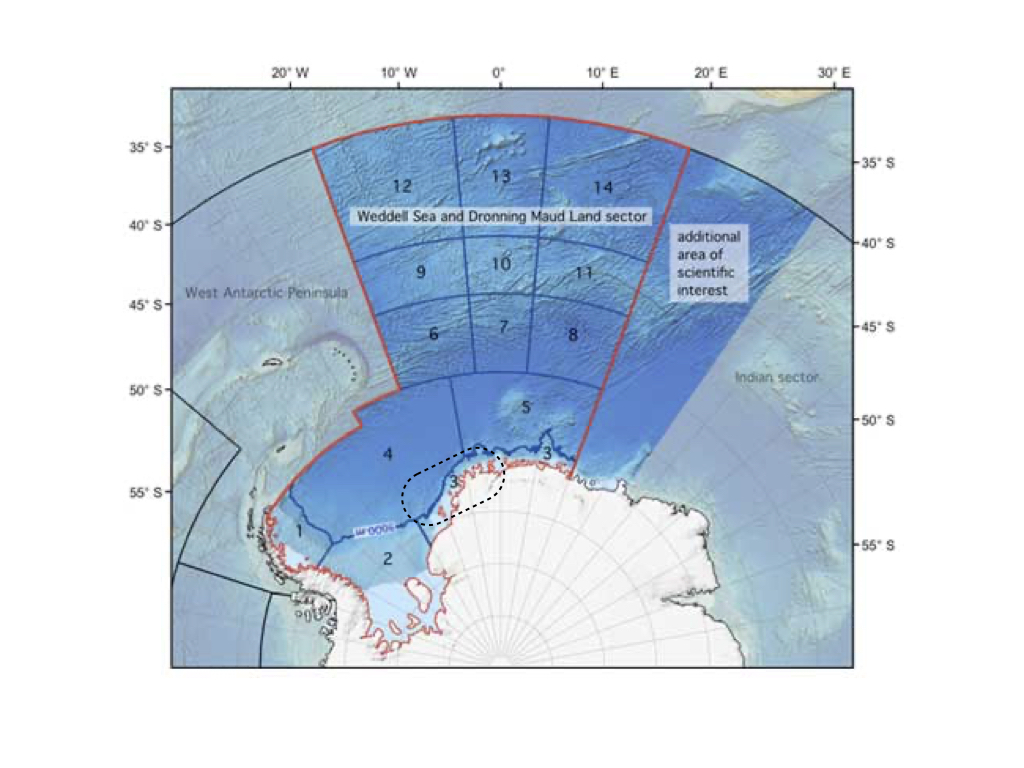
\includegraphics[width=12cm]{Fig.1_StudyMap} \caption{Map of the Weddell Sea and Dronning Maud Land sector highlighting with a dashed-line contour the high Antarctic shelf that represents the spatial extent of the food web. Modified from www.soos.aq.}\label{fig:unnamed-chunk-1}
\end{figure}

\clearpage

\begin{figure}
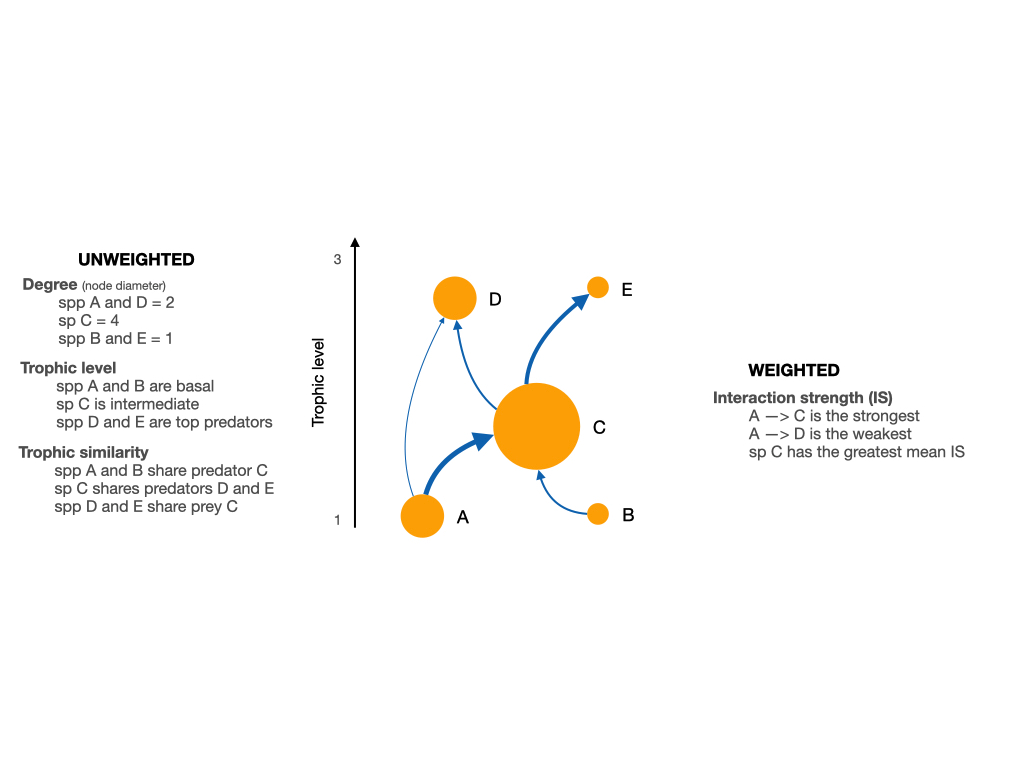
\includegraphics[width=12cm]{Fig.2_ToyFoodWeb} \caption{Scheme of a network showing the weighted and unweighted properties we used to characterize the species of the Weddell Sea food web. Directed arrows indicate the flow of energy; the width of the arrow represents the interaction strength of it.}\label{fig:unnamed-chunk-2}
\end{figure}

\clearpage

\begin{figure}
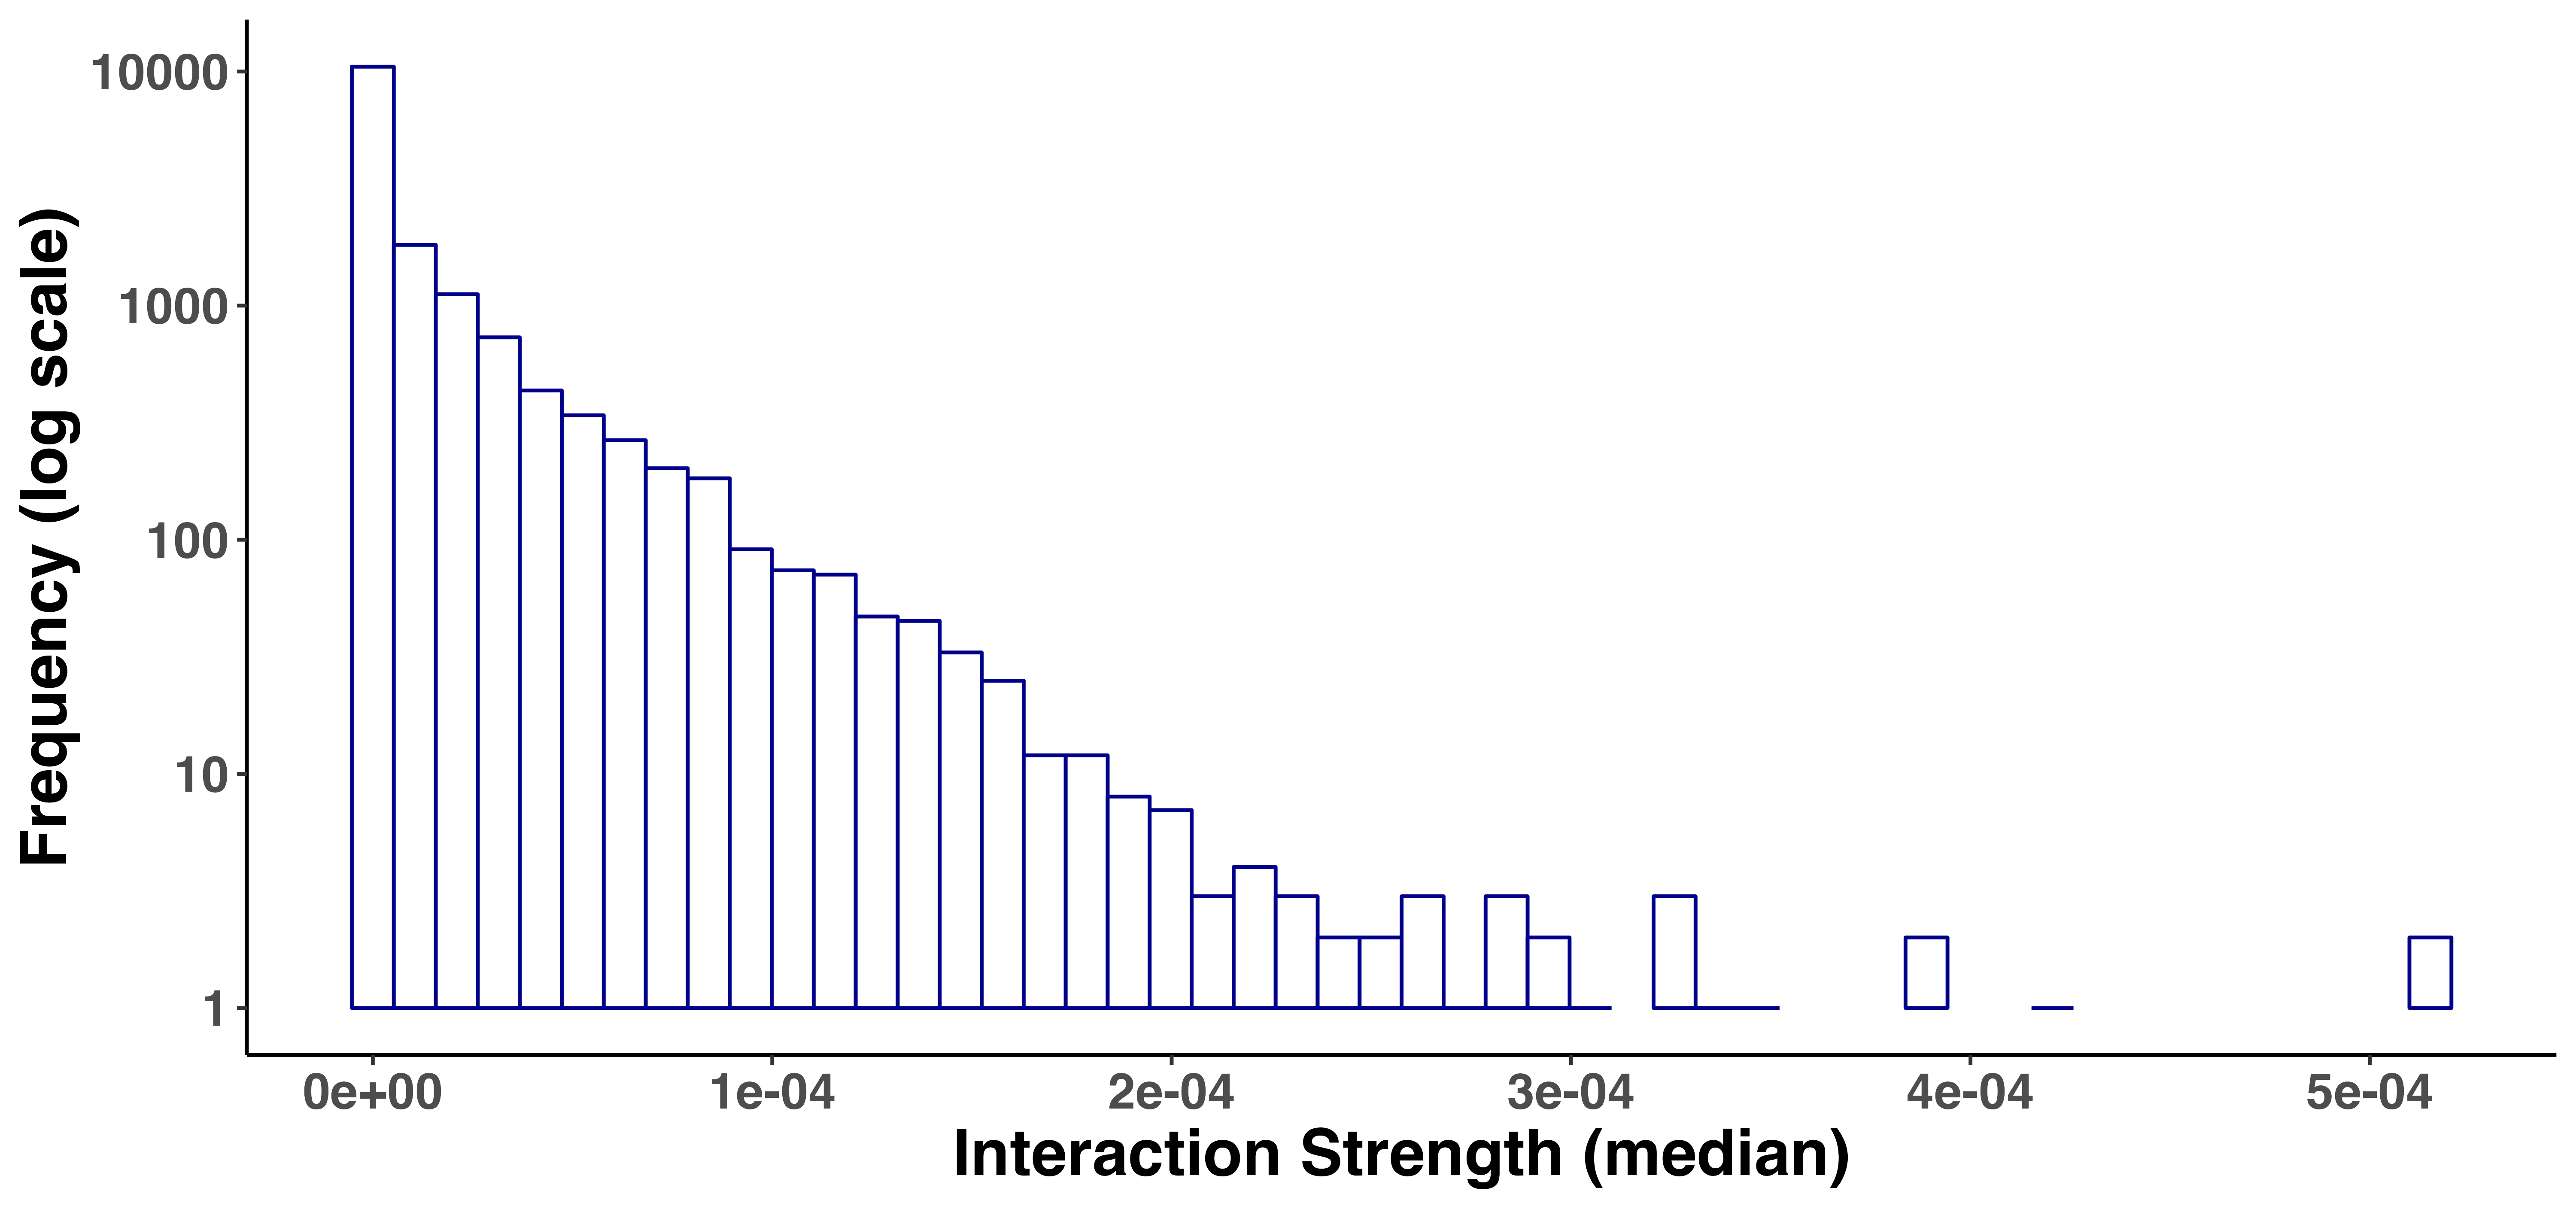
\includegraphics[width=12cm]{Fig3_IntDist_sim} \caption{Frequency distribution of (median) interaction strengths for the Weddell Sea food web. The distribution was best fitted to a 'log-Normal' model. Total number of interactions = 16041.}\label{fig:unnamed-chunk-3}
\end{figure}

\clearpage

\begin{figure}
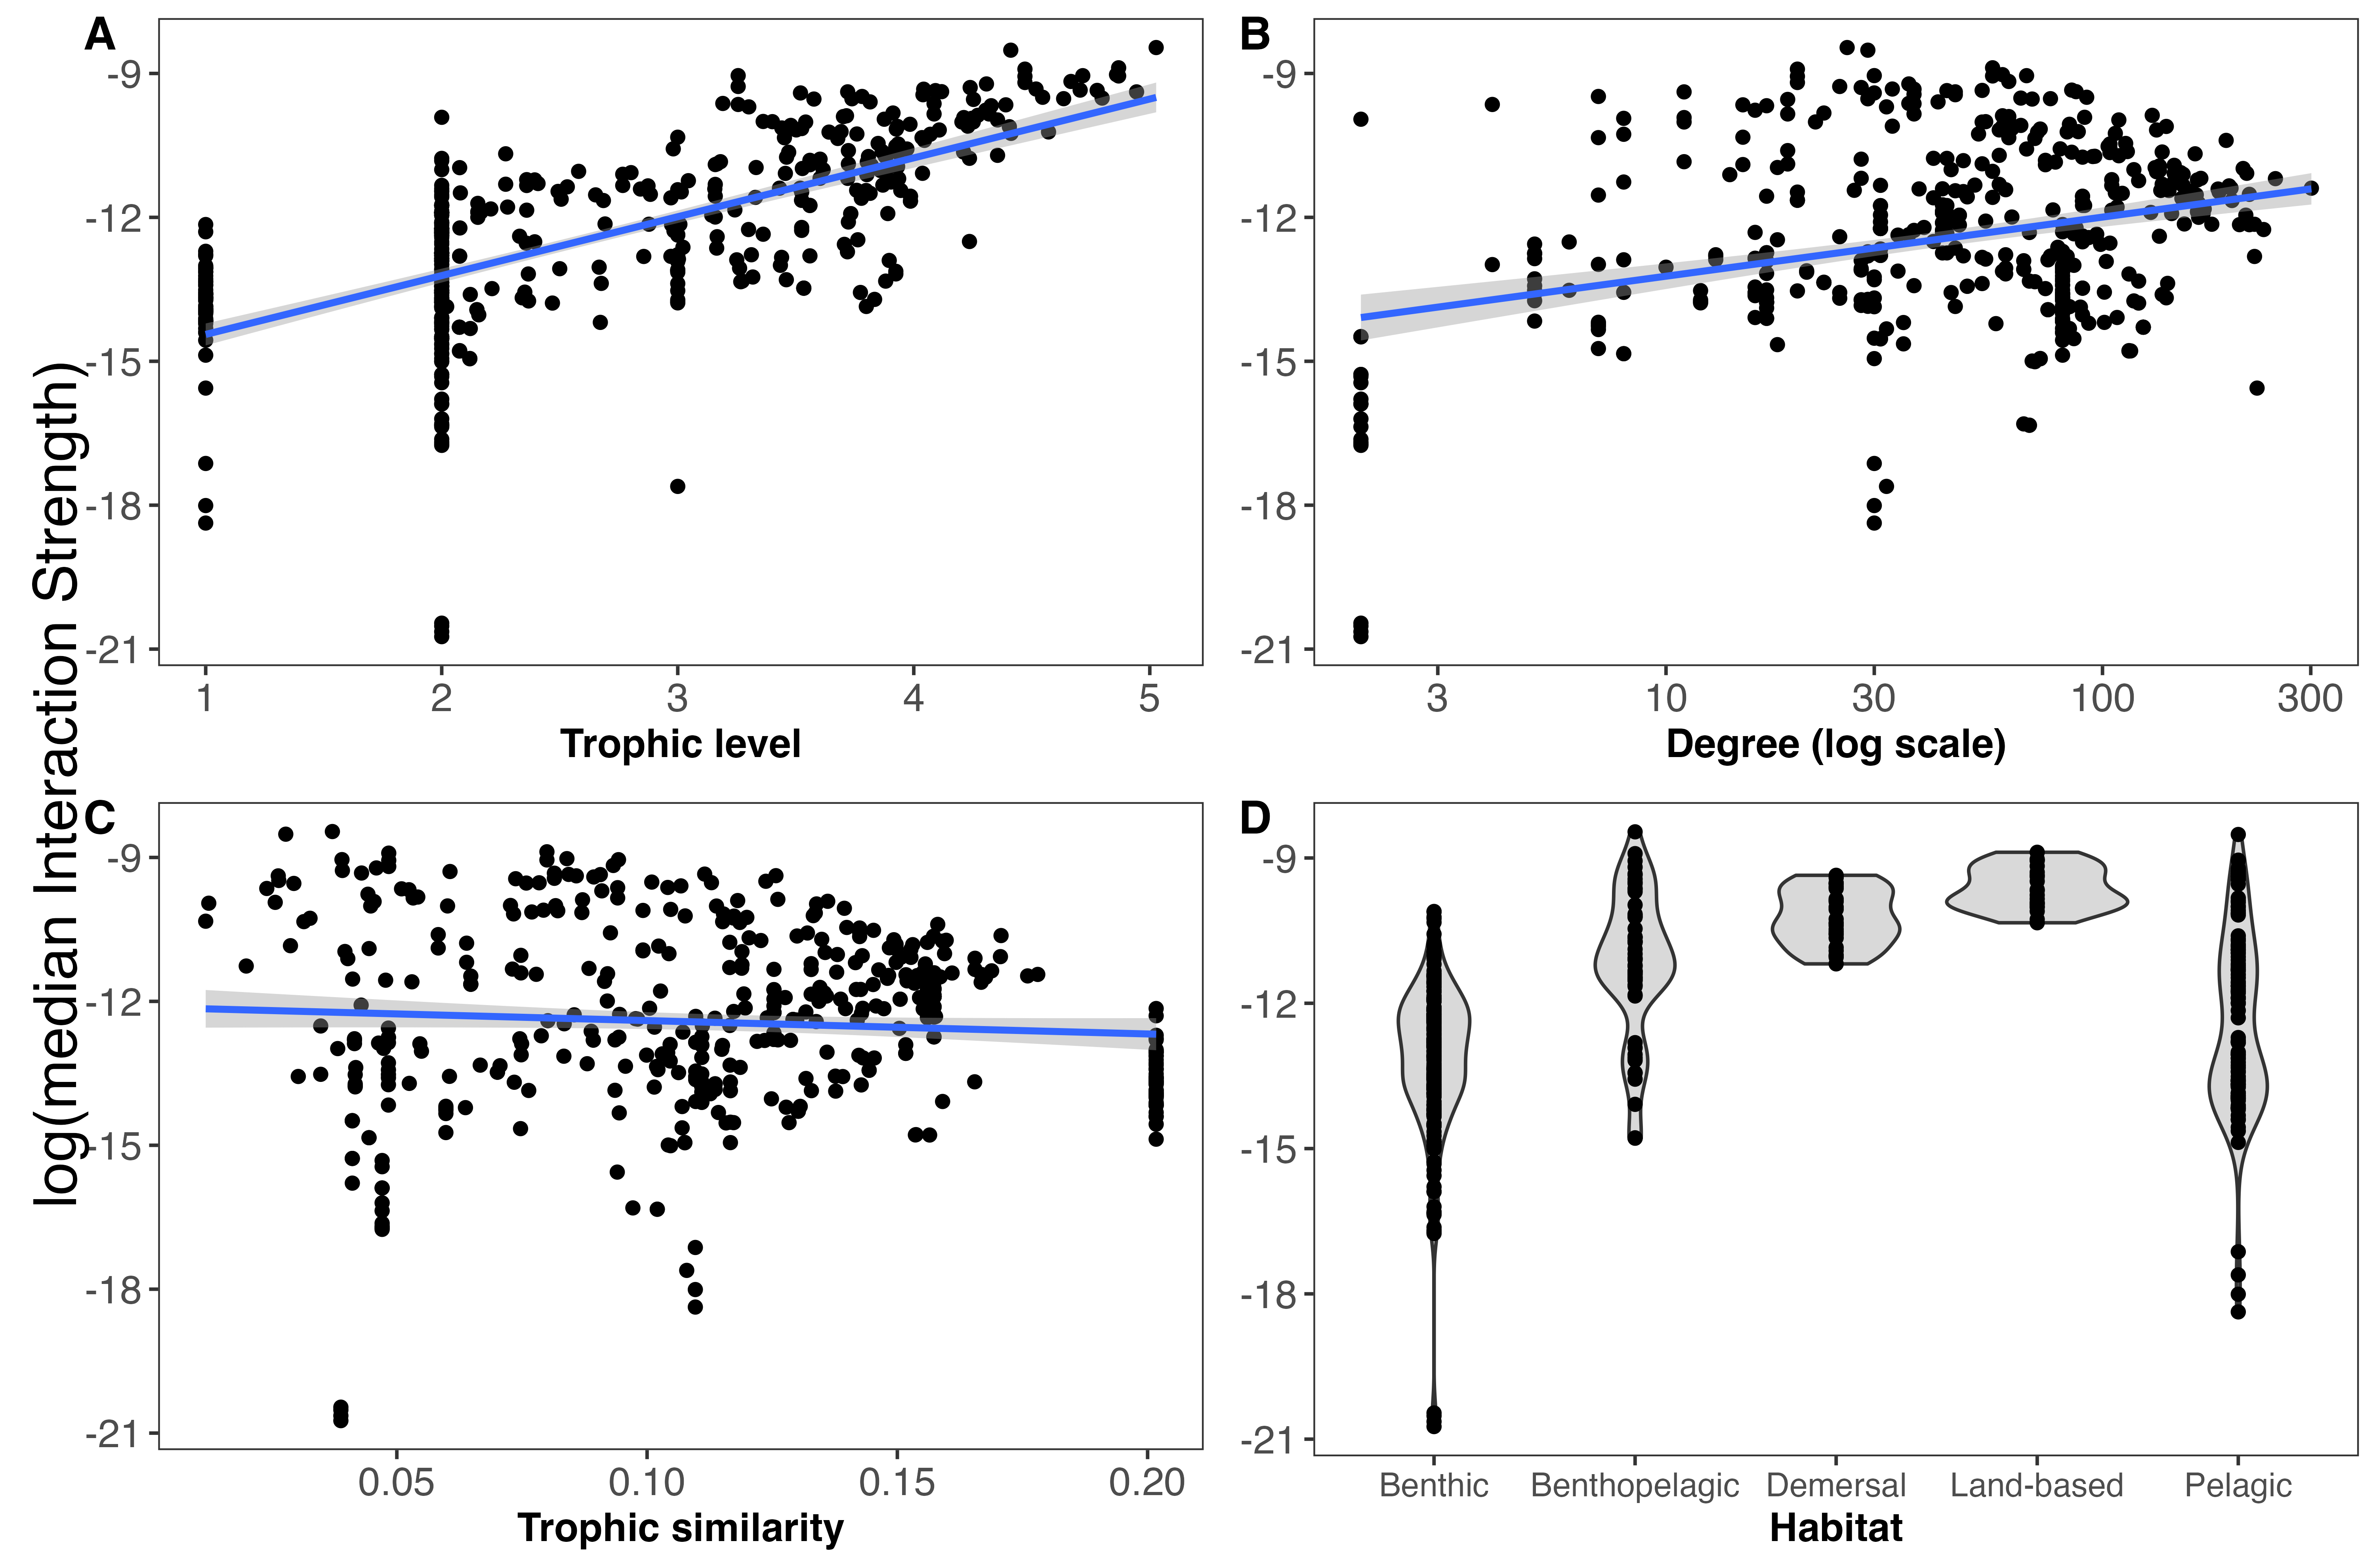
\includegraphics[width=12cm]{Fig4_LinReg_sim} \caption{Relationships between weighted (median Interaction Strength) and unweighted properties including habitat. Linear regressions are shown between log(median interaction strength) and trophic level (A), degree (B) and trophic similarity (C). Linear regressions for trophic level ($y = 1.23x - 15.67, R^2 = 0.46, p-value < 2.2e-16$), degree ($y = 0.006x - 12.86, R^2 = 0.03, p-value = 1.19e-4$) and trophic similarity ($y = -2.78x - 12.12, R^2 = 0.03, p-value = 0.11$).}\label{fig:unnamed-chunk-4}
\end{figure}

\clearpage

\begin{figure}
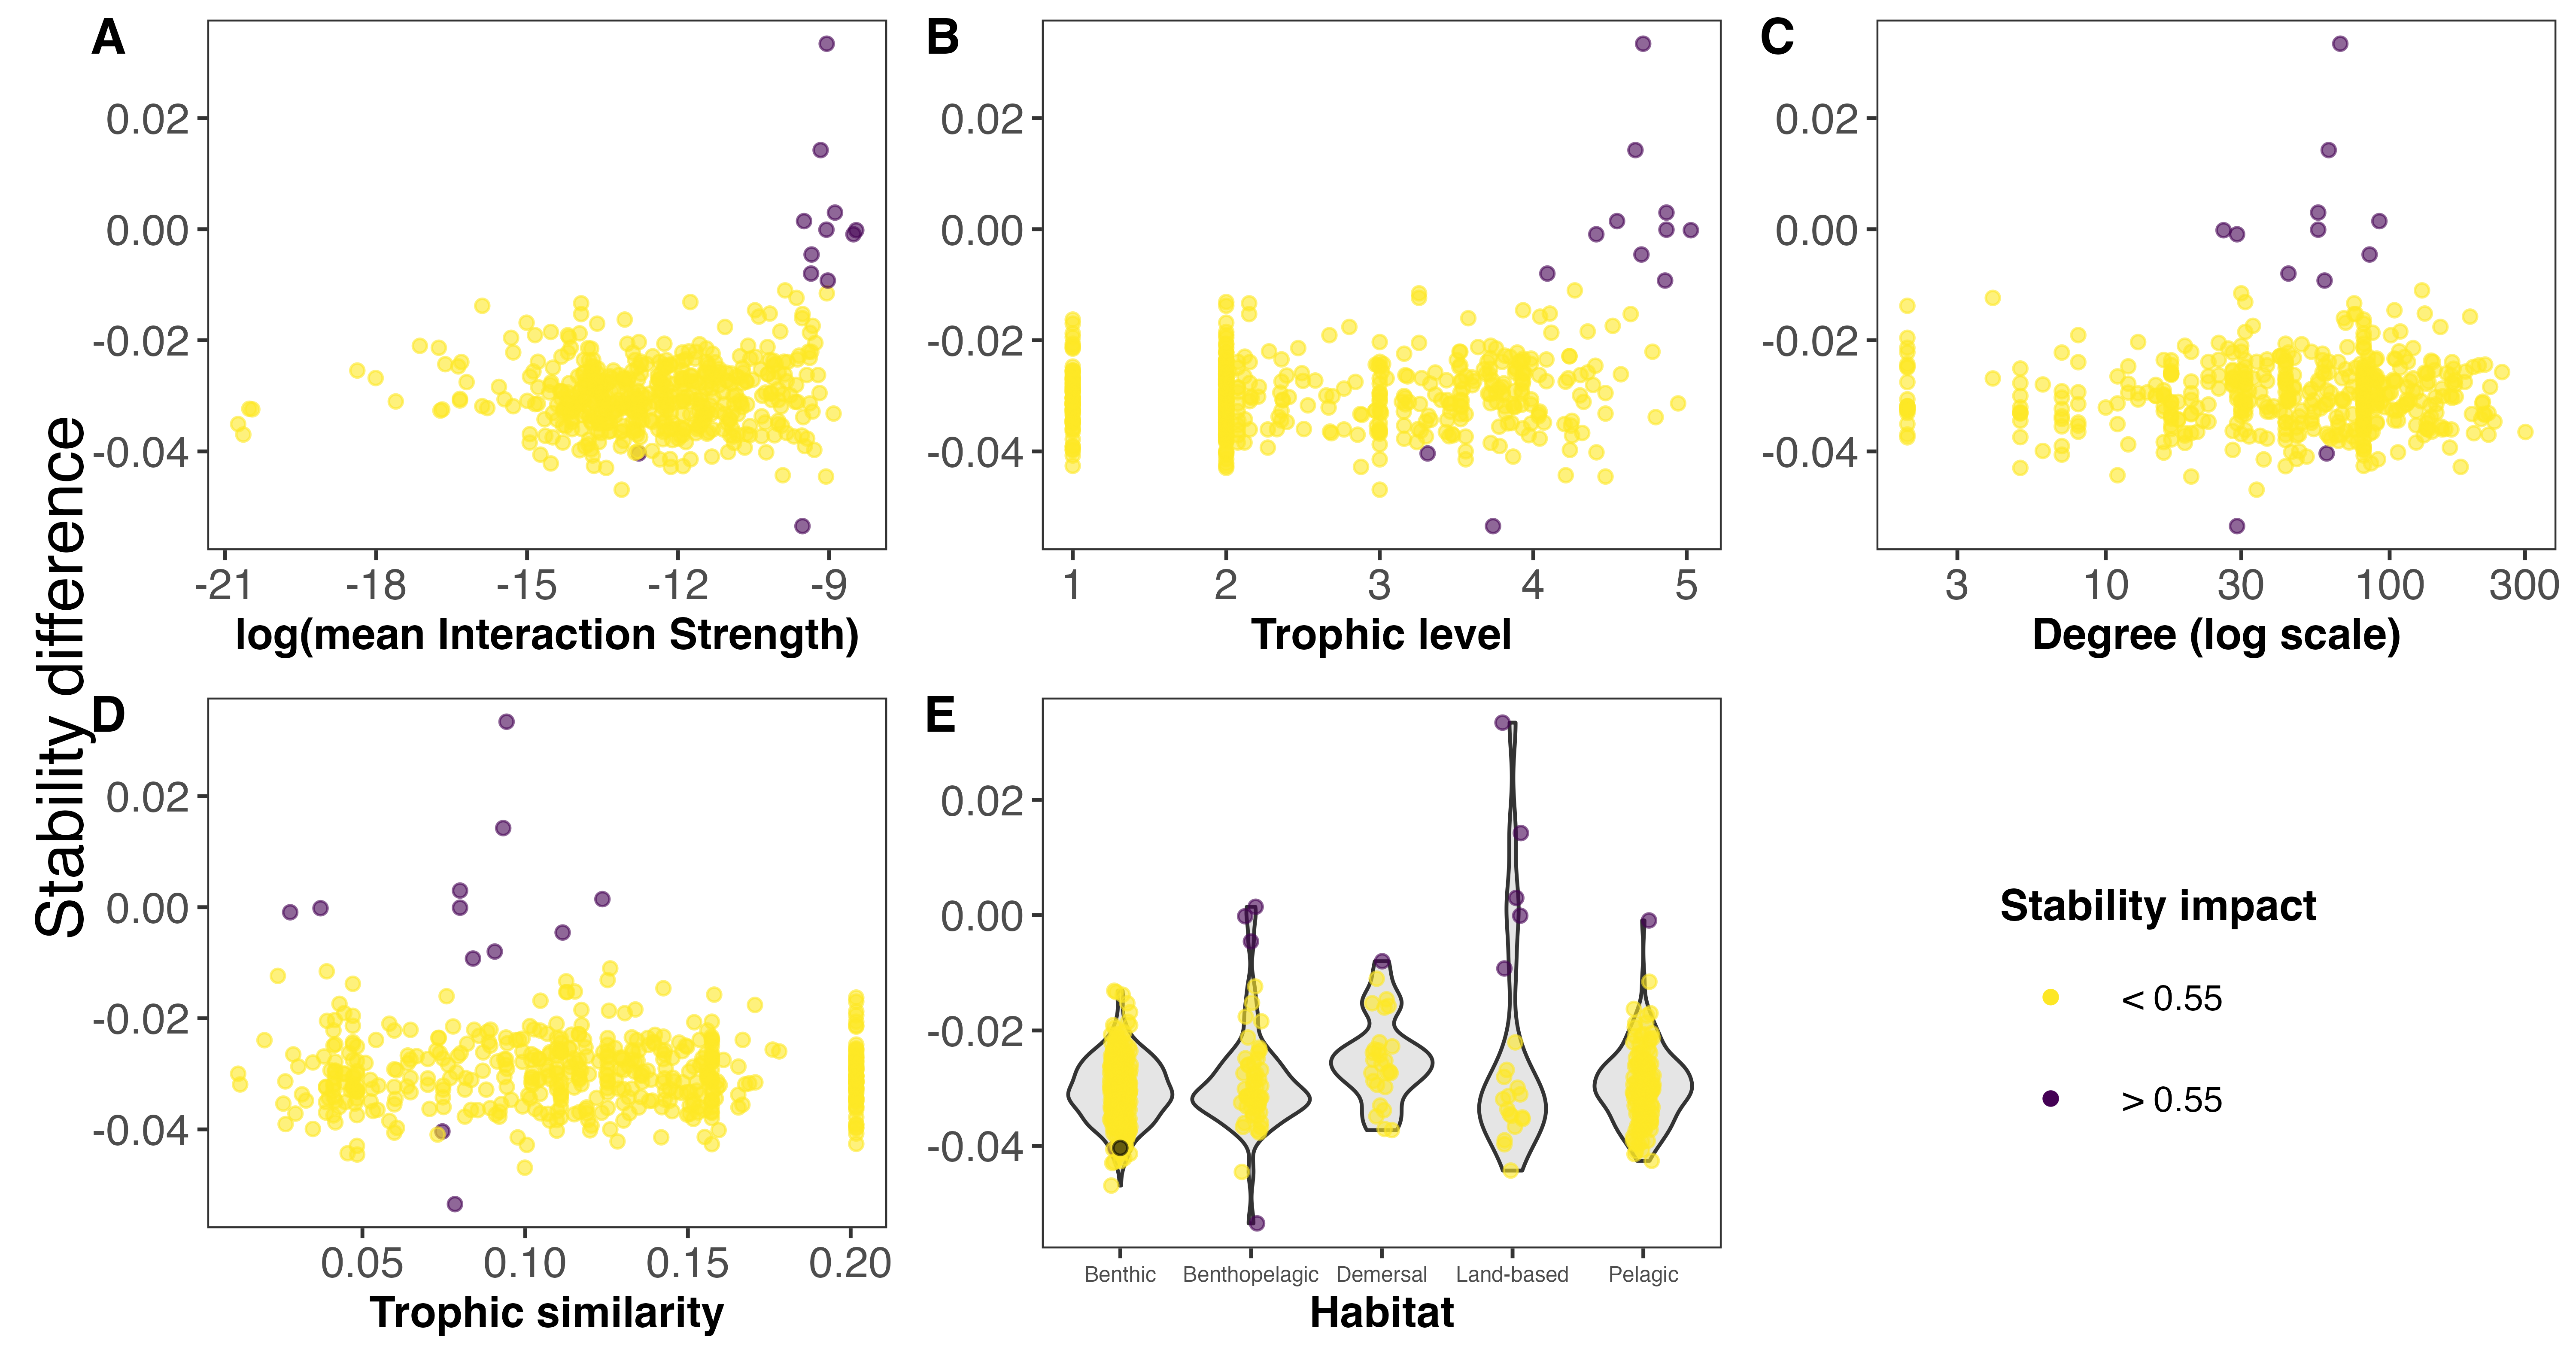
\includegraphics[width=12cm]{Fig.5_QSSDif} \caption{Stability  difference (median maximum eingenvalue) between the whole Weddell Sea food web (n = 490) and the food web minus one species (n = 489) for weighted (interaction strength) and unweighted species properties, and habitat. Point color indicates the impact on the stability; if substantial (> 0.55 relative difference) the extinction of that species altered the stability of the food web.}\label{fig:unnamed-chunk-5}
\end{figure}

\clearpage

\begin{table}[t]
\caption{Properties for the species with highest impact on the food web stability. Summary of maximum eigenvalue (QSS) distribution of differences before and after performing extinction simulations in the Weddell Sea food web. Ordered by decreasing proportion of positive differences. References: medianIS = median interaction strength, TL = trophic level, Deg = degree, TS = trophic similarity, Prop dif QSS + = Proportion of positive differences, Prop dif QSS - = Proportion of negative differences.}
\begin{tabular}{l c c c c c c c}
\tophline

\textbf{Species} & \textbf{medianIS} & \textbf{TL} & \textbf{Deg} & \textbf{TS} & \textbf{Habitat} & \textbf{Prop dif QSS +} & \textbf{Prop dif QSS -} \\
\middlehline
Hydrurga leptonyx & 1.162399e-04 & 4.716 & 67 & 0.09428900 & Land-based & 0.651 & 0.349 \\
\middlehline
Arctocephalus gazella & 1.021457e-04 & 4.666 & 61 & 0.09325095 & Land-based & 0.613 & 0.387 \\
\middlehline
Mirounga leonina & 1.314364e-04 & 4.868 & 56 & 0.07998706 & Land-based & 0.581 & 0.419 \\
\middlehline
Mesonychoteuthis hamiltoni & 1.966995e-04 & 4.411 & 29 & 0.02781001 & Pelagic & 0.573 & 0.427 \\
\middlehline
Orcinus orca & 1.557436e-04 & 5.027 & 26 & 0.03712293 & Benthopelagic & 0.570 & 0.430 \\
\middlehline
Macrourus holotrachys & 8.350777e-05 & 4.705 & 85 & 0.11150715 & Benthopelagic & 0.568 & 0.432 \\
\middlehline
Notothenia marmorata & 8.357614e-05 & 4.092 & 44 & 0.09065823 & Demersal & 0.563 & 0.437 \\
\middlehline
Macrourus whitsoni & 7.945909e-05 & 4.546 & 92 & 0.12372962 & Benthopelagic & 0.558 & 0.442 \\
\middlehline
Ommatophoca rossii & 1.124936e-04 & 4.868 & 56 & 0.07998706 & Land-based & 0.558 & 0.442 \\
\middlehline
Leptonychotes weddelli & 1.137129e-04 & 4.859 & 59 & 0.08397729 & Land-based & 0.551 & 0.449 \\
\middlehline
Aporocidaris milleri & 2.762191e-06 & 3.312 & 60 & 0.07457218 & Benthic & 0.447 & 0.553 \\
\middlehline
Balaenoptera acutorostrata & 5.181120e-05 & 3.738 & 29 & 0.07843173 & Benthopelagic & 0.423 & 0.577 \\
\bottomhline
\end{tabular}
\end{table} 

\appendixfigures
\clearpage

\begin{figure}
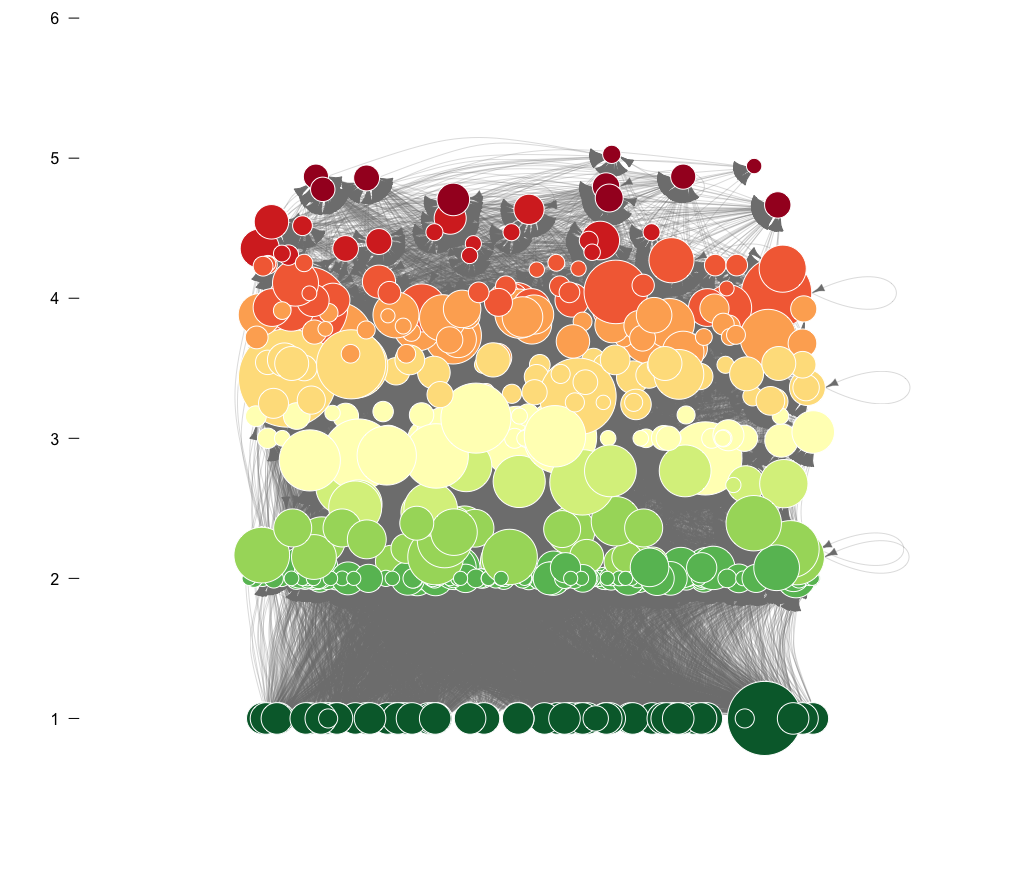
\includegraphics[width=12cm]{App1_FWplot} \caption{Graphic representation of the Weddell Sea food web. Species (nodes) are arranged vertically and colored by trophic level. The diameter of the node indicates the total number of interactions. Predator-prey interactions are represented by the arrows, from prey to predator.}\label{fig:unnamed-chunk-6}
\end{figure}






%%%%%%%%%%%%%%%%%%%%%%%%%%%%%%%%%%%%%%%%%%
%% optional

%%%%%%%%%%%%%%%%%%%%%%%%%%%%%%%%%%%%%%%%%%

%%%%%%%%%%%%%%%%%%%%%%%%%%%%%%%%%%%%%%%%%%
\authorcontribution{TIM and LAS: Conceptualization (lead); Data curation
(lead); Formal analysis (lead); Methodology (lead); Coding (lead);
Writing -- original draft (lead); Writing -- review and editing (lead).
SK: Conceptualization (lead); Formal analysis (supporting); Methodology
(supporting); Coding (supporting); Writing -- original draft
(supporting); Writing -- review and editing
(supporting).} %% optional section

%%%%%%%%%%%%%%%%%%%%%%%%%%%%%%%%%%%%%%%%%%
\competinginterests{The authors declare no competing
interests.} %% this section is mandatory even if you declare that no competing interests are present

%%%%%%%%%%%%%%%%%%%%%%%%%%%%%%%%%%%%%%%%%%

%%%%%%%%%%%%%%%%%%%%%%%%%%%%%%%%%%%%%%%%%%
\begin{acknowledgements}
We thank all persons that dedicated time to build and curate the dataset
GATEWAy that enable us to carry out this work. We also thank the
organizers of the different virtual workshops of the Weddell Sea and
Droning Maud Land (WSDML) Regional Working Group for giving us the
possibility to participate and contribute in the Special Issue.
\end{acknowledgements}

%% REFERENCES
%% DN: pre-configured to BibTeX for rticles

%% The reference list is compiled as follows:
%%
%% \begin{thebibliography}{}
%%
%% \bibitem[AUTHOR(YEAR)]{LABEL1}
%% REFERENCE 1
%%
%% \bibitem[AUTHOR(YEAR)]{LABEL2}
%% REFERENCE 2
%%
%% \end{thebibliography}

%% Since the Copernicus LaTeX package includes the BibTeX style file copernicus.bst,
%% authors experienced with BibTeX only have to include the following two lines:
%%
\bibliographystyle{copernicus}
\bibliography{WeddellSea.bib}
%%
%% URLs and DOIs can be entered in your BibTeX file as:
%%
%% URL = {http://www.xyz.org/~jones/idx_g.htm}
%% DOI = {10.5194/xyz}


%% LITERATURE CITATIONS
%%
%% command                        & example result
%% \citet{jones90}|               & Jones et al. (1990)
%% \citep{jones90}|               & (Jones et al., 1990)
%% \citep{jones90,jones93}|       & (Jones et al., 1990, 1993)
%% \citep[p.~32]{jones90}|        & (Jones et al., 1990, p.~32)
%% \citep[e.g.,][]{jones90}|      & (e.g., Jones et al., 1990)
%% \citep[e.g.,][p.~32]{jones90}| & (e.g., Jones et al., 1990, p.~32)
%% \citeauthor{jones90}|          & Jones et al.
%% \citeyear{jones90}|            & 1990


\end{document}
